%\hypertarget{aula-12}{%
%\chapter{Aula: 12}\label{aula-12}}




\hypertarget{continuauxe7uxe3o-transport-layer}{%
\chapter{Continuação: Transport Layer}\label{continuauxe7uxe3o-transport-layer}}

Como citado na aula anterior, o protocolo \emph{stop and wait}, no qual
o envio do próximo segmento (também é chamado de pacote por uma questão
histórica) ocorre somente após o recebimento da resposta do segmento
anterior, é uma forma ineficiente para a transferência de dados
confiáveis (\emph{reliable data transfer}, rdt) pois, após a transmissão
de um segmento, os recursos disponíveis para a conexão ficarão ociosos
até a chegada da resposta do segmento enviado. Dessa maneira,
objetivando o aumento da eficiência do mesmo, fora propostos duas
soluções: \emph{Go-Back-N} (GBN); e \emph{selective repeat}

\hypertarget{go-back-n}{%
\subsection{GO-BACK-N}\label{go-back-n}}

A ideia do protocolo GBN é baseado em um subconjunto de N elementos da
fila de transmissão (um dos motivos para a imposição de um tamanho
limite é o controle de fluxo). Os elementos dessa fila são compostos por
espaços que podem ser preenchidos por segmentos oriundo das camadas
superiores. Esse subconjunto, chamado de janela, contém os espaços
preenchidos por segmentos enviados mas sem confirmação
(\emph{acknowledged}) e espaços ainda não preenchidos. Ao receber uma
resposta, o espaço relacionado ao respectivo segmentos sai da janela, um
novo elemento da fila de transmissão é adicionado, gerando o efeito de
deslizar da janela para a direita na fila de transmissão. Devido a esse
efeito o GBN é chamado de \emph{sliding-window protocol}.

Caso todos os espaços disponibilizados pela janela estejam preenchidos,
novos dados não poderão ser aceitos, retornando às camadas superiores,
sendo esse retorno uma indicação de indisponibilidade.

Na metade superior da Figura \ref{Go-Back-N} podem ser reconhecidos os parâmetros:
\texttt{base}, que identifica o valor inicial incluído;
\texttt{nextseqnum}, referente ao próximo elemento a ser enviado; e
\texttt{send\ window\ size}, tamanho da janela (valor do N supracitado).
A metade inferior mostra o registro dos eventos ocorridos durante o
protocolo.

\begin{figure}[h!]
\centering
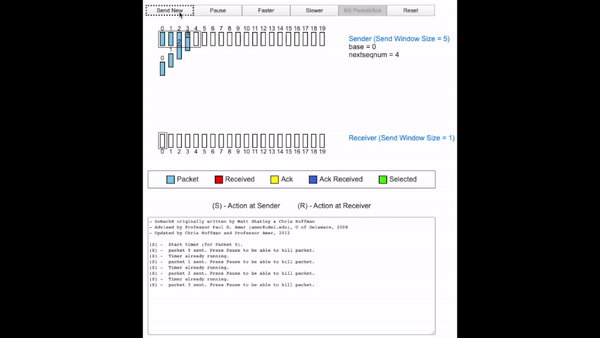
\includegraphics[keepaspectratio, width=12cm, height=9cm]{imagens/12/12 - GBN.png}
\caption{Go-Back-N \\
Disponível em:
https://media.pearsoncmg.com/aw/ecs\_kurose\_compnetwork\_7/cw/
content/interactiveanimations/go-back-n-protocol/index.html \\}
\label{Go-Back-N}
\end{figure}



Como o envio dos segmentos é feito em ordem, é esperado que os
respectivos ACK's sejam recebidos em ordem (\emph{cumulative
acknowledgment}). Caso o \emph{server} receba um segmento corrompido ou
fora de ordem, o mesmo é descartado e um ACK referente ao último
segmento íntegro ordenado é disparado. O ACK duplicado recebido é
descartado. Da perspectiva do \emph{client}, a não recepção ACK
correspondente ao segmento enviado, pode resultar em dois casos.
Primeiro, se a recepção do ACK `x + 1' ocorrer, porém a do `x' não, o
GBN considerará que o segmento `x' foi recebido corretamente pelo
\emph{server} e o seu ACK fora perdido durante a transmissão, marcando,
portanto, o segmento `x' como enviado corretamente. O segundo caso é a
respeito da não recepção de respostas dentro de um período
predeterminado (\emph{timeout}), algo que resulta na retransmissão dos
segmentos relativos.

Exemplo 1:

\begin{enumerate}
\def\labelenumi{\arabic{enumi}.}
\tightlist
\item
  \emph{cliente} dispara 5 segmentos (1, 2, 3, 4, 5)
\item
  \emph{server} recebe o segmento número 2 corrompido
\item
  \emph{server} dispara os seguintes ACK's: 1, 1, 1, 1, 1
\item
  \emph{cliente} recebe 5 ACK's referentes ao segmento 1, indicando a
  necessidade de retransmissão dos segmentos 2, 3, 4 e 5.
\end{enumerate}

Exemplo 2:

\begin{enumerate}
\def\labelenumi{\arabic{enumi}.}
\tightlist
\item
  \emph{client} dispara 5 segmentos (1, 2, 3, 4, 5)
\item
  \emph{server} recebe todos os segmentos corretamente
\item
  \emph{server} dispara os seguintes ACK's: 1, 2, 3, 4, 5
\item
  \emph{client} somente o ACK número 5, tendo, o resto, sido perdido
  durante a transmissão.
\item
  \emph{client} qualifica todos os 5 segmentos como tendo sido recebidos
  corretamente pelo \emph{server}
\end{enumerate}

\hypertarget{selective-repeat-sr}{%
\subsection{Selective Repeat (SR)}\label{selective-repeat-sr}}

É importante perceber, como mostrado no Exemplo 1, que um único elemento
corrompido pode causar a retransmissão de uma série de segmentos,
tornando, assim, o GBN ineficiente para esses casos. O aumento dessa
ineficiência é diretamente proporcional ao número de erros provocados
pelo canal de transmissão.

O protocolo \emph{Selective Repeat} (SR), como o próprio nome já induz,
tem o objetivo de diminuir o número de retransmissões desnecessárias.
Para tal, utiliza um subconjunto de N elementos da fila de transmissão,
chamada de janela, com cada elemento sendo um espaço que pode ser
preenchido por um segmento e marcado como não usável, usável, enviado e
confirmado, algo análogo ao GBN. Porém, diferencia-se pelo seu
comportamento, como mostrado na Figura \ref{Selective Repeat}.


\begin{figure}[h!]
\centering
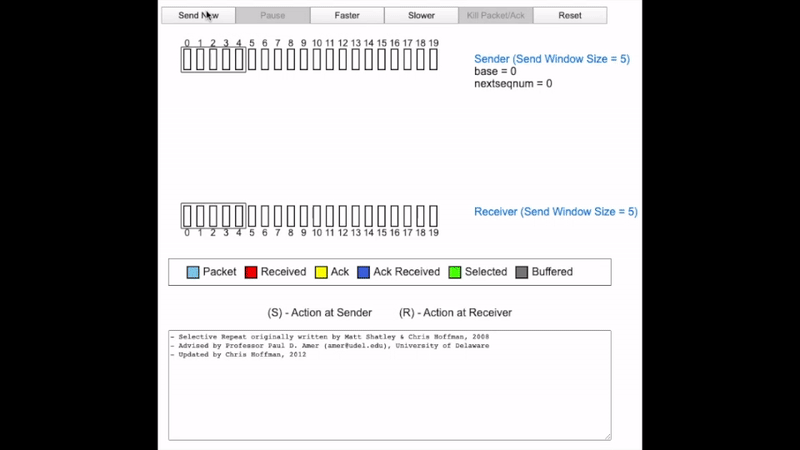
\includegraphics[keepaspectratio, width=12cm, height=9cm]{imagens/12/12 - animation of selective repeat.png}
\caption{Selective Repeat \\
Disponível em:
https://media.pearsoncmg.com/aw/ecs\_kurose\_compnetwork\_7/cw/content/interactiveanimations/selective-repeat-protocol/index.html \\}
\label{Selective Repeat}
\end{figure}



\begin{enumerate}
\def\labelenumi{\arabic{enumi}.}
\tightlist
\item
  um elemento só é marcado como confirmado quando o mesmo receber seu
  respectivo ACK.
\item
  a janela desloca-se somente após o recebimento do ACK relativo ao
  elemento na posição \texttt{base}, localizado no início da janela.
\item
  o \emph{server} enviará um ACK para cada segmento mesmo se ele estiver
  fora de ordem (mas dentro das condições citadas a seguir).
\item
  o \emph{client} terá uma janela própria (do mesmo tamanho da janela do
  \emph{client}), organizando-a, também, com 4 marcadores: esperado;
  fora de ordem; aceitado; não usável.
\item
  um segmento recebido fora de ordem não será descartado e sim
  armazenado em uma memória temporária (\emph{buffer}) (novamente,
  dentro das condições citadas a seguir).
\end{enumerate}

Esse comportamento gera uma possível dessincronização da posição das
janelas do \emph{cliente} e do \emph{server}, pois o \emph{server} pode
receber adequadamente um segmento mas o seu ACK relativo ter sido
corrompido ou perdido durante a transmissão. O pior caso de
dessincronização ocorre quando todos os ACK's enviados tenham sido
perdidos e, consequentemente, o \emph{server} estará adiantado em
\texttt{N} elementos. Assim, caso o \emph{server} receba um segmento com
o número da sequência entre entre os intervalos:



\begin{enumerate}
\def\labelenumi{\arabic{enumi}.}
\tightlist
\item
    \texttt{[`base`, `base` + `N` - 1]: armazenar em memória temporária e enviar o ACK.}
\item
    \texttt{[`base`-N, `base` - 1]: reenviar o ACK.}
\item
  Fora dos anteriores: ignorar.
\end{enumerate}

A dessincronização pode causar a recepção de um segmento já recebido,
gerando um dilema para o receptor: o segmento recebido é novo ou é uma
retransmissão ?

Essa possível dessincronização pode causar um dilema para o receptor dos
dados, pois, como mostrado na A Figura \ref{Dilema do Selective Repeat} mostra o dilema ocasionado
pela possível dessincronização: os dados recebidos são derivados de uma
retransmissão, como mostrado em (a), ou de um novo segmento (b)?

\begin{figure}[h!]
\centering
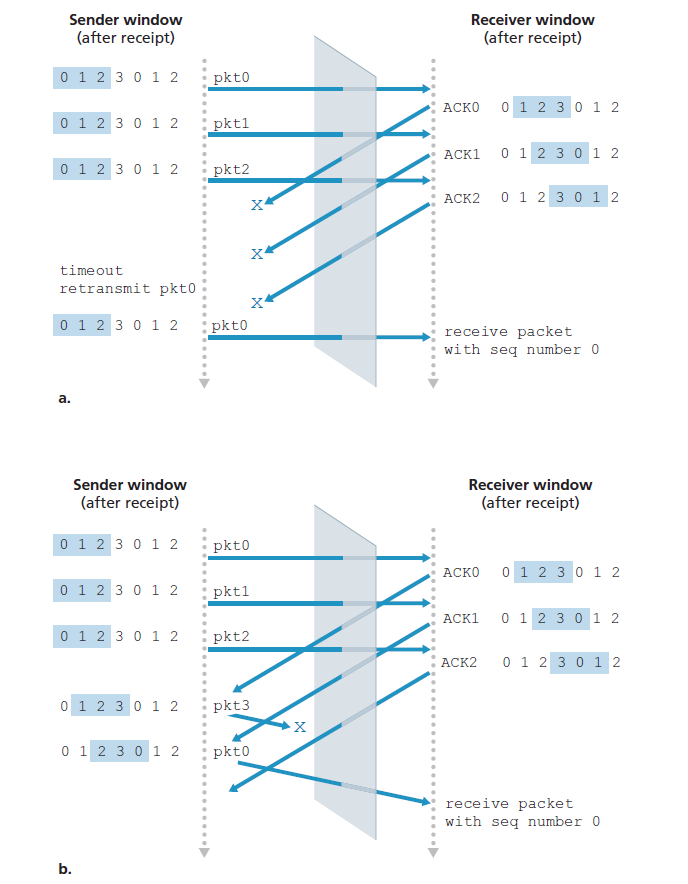
\includegraphics[keepaspectratio, width=18cm, height=15cm]{imagens/12/12 - Dilema do Selective Repeat.png}
\caption{Dilema do Selective Repeat \\
Imagem retirada de: Computer Networking a top-down approach. 8th
ed.~Pearson, página 225. \\}
\label{Dilema do Selective Repeat}
\end{figure}


Colocações importantes:

\begin{enumerate}
\def\labelenumi{\arabic{enumi}.}
\tightlist
\item
  O número de sequência é um valor finito determinado pelo número de
  bits disponibilizados para tal.
\item
  O \emph{buffer} do receptor deve poder armazenar 2 janelas, ou seja, o
  seu tamanho deve ser, no mínimo, o dobro do \texttt{window\ size}
  (\texttt{N}).
\item
  O \texttt{N} é determinado durante o \emph{handshaking}, limitado pelo
  tamanho do \emph{buffer} do receptor (como citado em 2).
\end{enumerate}

\hypertarget{tcp}{%
\subsection{TCP}\label{tcp}}

A camada de aplicação (\emph{application layer}), para o envio de um
arquivo, conta com os serviços de transmissão de dados confiáveis
fornecidos pelo \emph{Transmission Control Protocol} (TCP), protocolo da
camada de transporte. O TCP, ao receber o arquivo oriundo da
\emph{application layer}, divide-o em pedaços de comprimentos iguais
chamados de \emph{chunk's of data} (com exceção do último, normalmente
menor), de tamanho igual ao MSS (\emph{maximum segment size}),
normalmente de 1460 \emph{bytes}. O encapsulamento de um \emph{chunk of
data}, etapa que une o mesmo com o \emph{header} do TCP, resulta em um
conjunto de dados chamado de segmento.

O parâmetro MSS é determinado pelo MTU (\emph{Maximum Trasmission
Unit}), tamanho máximo do \emph{frame} da camada de enlace
(\emph{link-layer}), que tem como objetivo garantir que o segmento TCP
somado com o \emph{header} do TCP/IP (tipicamente 40 bytes), caberá no
\emph{frame} do \emph{link-layer}.

Após sua formação, o segmento é inserido no \emph{send buffer}, memória
temporária destinada ao envio dos dados para as camadas inferiores. Essa
memória é acessada de tempos em tempos para o envio dos segmentos ali
presentes.

Porém, diferente do UDP, o TCP é um protocolo orientado à conexão
(\emph{connection-oriented}), pois o primeiro contato entre dois
dispositivos ocorre com base no procedimento \emph{3-way handshake}, o
qual visa assegurar à confiabilidade na transmissão dos dados a partir
da definição dos parâmetros da conexão. O \emph{3-way handshake} é
caracterizado pela transmissão de 3 segmentos especiais. O primeiro é
emitido pelo \emph{client} visando o início da conexão. O segundo é uma
resposta do \emph{server}, indicando que o segmento foi recebido
corretamente. Por fim, o \emph{client} confirma que também recebeu o
segmento oriundo do \emph{server}. Os dois primeiros segmentos especiais
não contém dados, mas o terceiro pode conter.

A seguir está listado as características principais do TCP (mencionado
em aulas anteriores):

\begin{enumerate}
\def\labelenumi{\arabic{enumi}.}
\tightlist
\item
  Ponto-a-ponto
\item
  Transmissão de confiança, com fluxo de dados ordenado
\item
  \emph{Full Duplex}: fluxo de dados bi-direcional na mesma conexão
\item
  \emph{cumulative} ACK's
\item
  \emph{Pipelining}: controle de fluxo e congestionamento
\item
  \emph{Connection-oriented}
\item
  Fluxo controlado: o emissor não irá sobrecarregar o receptor
\end{enumerate}

\hypertarget{estrutura-do-segmento-tcp}{%
\subsubsection{Estrutura do segmento TCP}\label{estrutura-do-segmento-tcp}}

Como citado anteriormente, o segmento do TCP é composto por seu
\emph{header} e pelo pedaço do dado enviado pela camada de aplicação. O
\emph{header} é a sessão do segmento responsável pelos parâmetros de
conexão. São eles:

\begin{enumerate}
\def\labelenumi{\arabic{enumi}.}
\tightlist
\item
  números das portas de origem e destino, utilizados na multiplexação e
  demultiplexação, respectivamente.
\item
  \emph{checksum field}, importante na validação da integralidade dos
  dados recebidos
\item
  32-bit \emph{sequence number field}
\item
  32-bit \emph{acknowledgment number field}
\item
  16-bit \emph{receiver window}: usado para \emph{flow control}, indica
  o número de bytes que o receptor está disposto a aceitar
\item
  4-bit \emph{header length field}: especifica o tamanho do
  \emph{header} do TCP (como, normalmente, o \emph{options field} não é
  populado, o tamanho típico do \emph{header} é de 20 \emph{bytes})
\item
  \emph{options field}: é útil para a negociação do MSS entre outros.
\item
  \emph{flag field}: campo que contém 6 bits 8.1. bit ACK: indica a
  validade do campo ACK 8.2. bits RST, SYN e FIN: são usados para
  configuração das conexões 8.3. bits CWR e ECE: notificações de
  congestionamento 8.4. bit PSH: indica que o receptor deve repassar, de
  imediato, os dados recebidos para as camadas superiores 8.5. bit URG:
  marcado pela camada de aplicação do emissor, indica que há dados
  urgentes (Na prática, os bits PSH e URG não são usados)
\end{enumerate}

A Figura \ref{Estrutura do segmento TCP} mostra toda a estrutura do segmento TCP.


\begin{figure}[h!]
\centering
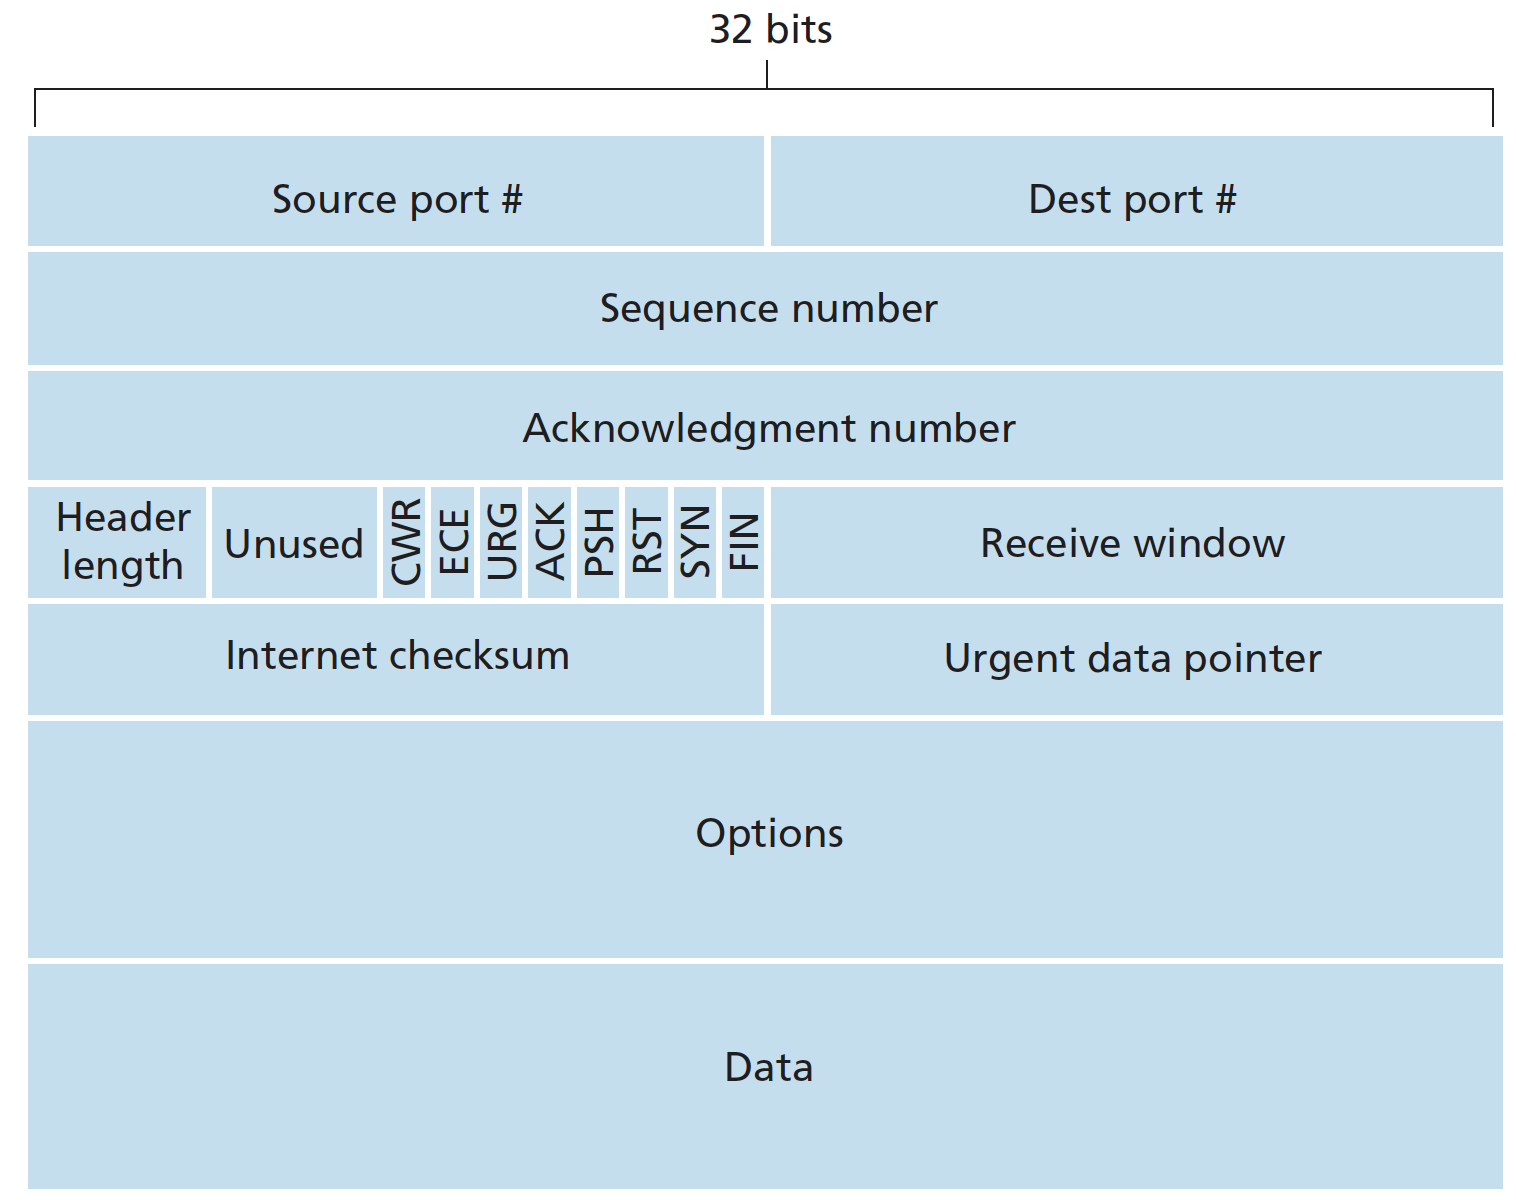
\includegraphics[keepaspectratio, width=12cm, height=9cm]{imagens/12/12 - Estrutura segmento TCP.png}
\caption{Estrutura do segmento TCP \\
Imagem retirada de: Computer Networking a top-down approach. 8th
ed.~Pearson, página 231. \\}
\label{Estrutura do segmento TCP}
\end{figure}



\hypertarget{sequuxeancia-e-ack}{%
\ssubsection{Sequência e ACK}\label{sequuxeancia-e-ack}}

O TCP vê os dados como um conjunto ordenado e não estruturado de fluxo
(\emph{stream}) de bytes, de forma que o \emph{sequence number} é uma
referência à ordem dos bytes (mais especificamente, a ordem do primeiro
\emph{byte} dos dados do segmento) e não da série de segmentos enviados.
Assim, para um arquivo de 500.000 \emph{bytes} (500 kB) e um MSS de
1.000 bytes (1 kB) serão construídos 500 segmentos, com o primeiro
assumindo o \emph{sequence number} de 0, o segundo 1000, o terceiro
2000, e assim em diante.

Já \emph{acknowledgment number} (ACK \emph{number}) é relativo ao
\emph{sequence number} do próximo \emph{byte}. Seguindo o exemplo
anterior, está contido, no primeiro segmento, 1000 bytes, e o seu
\emph{sequence number} é de 0 (portanto existem nesse segmento os
\emph{bytes} 0 até 999). Assim, após a chegada no \emph{byte} 999, o
receptor enviará a confirmação da recepção desse segmento com o
\emph{acknowledgment number} de 1000 (byte seguinte ao último recebido).
Dessa maneira, como o receptor só confirma (\emph{acknowledges}) o
primeiro byte ausente, no caso, o byte 1000, o protocolo TCP é dito como
provedor de \emph{cumulative acknowledgments}.

A Figura \ref{Sequence number e ACK} mostra um exemplo de como a variação do \emph{sequence number} e do \emph{acknowledgment number} ocorrem com o MSS de 1
\emph{byte} no Telnet. O \emph{Host A} envia seu \emph{byte} 42
(\emph{sequence number}) requisitando (ACK) o byte de \emph{sequence
number} 79 do \emph{Host B}, e o \emph{Host B} responde com o seu
\emph{byte} 79 e requisita o \emph{byte} 43 do \emph{Host A}.


\begin{figure}[h!]
\centering
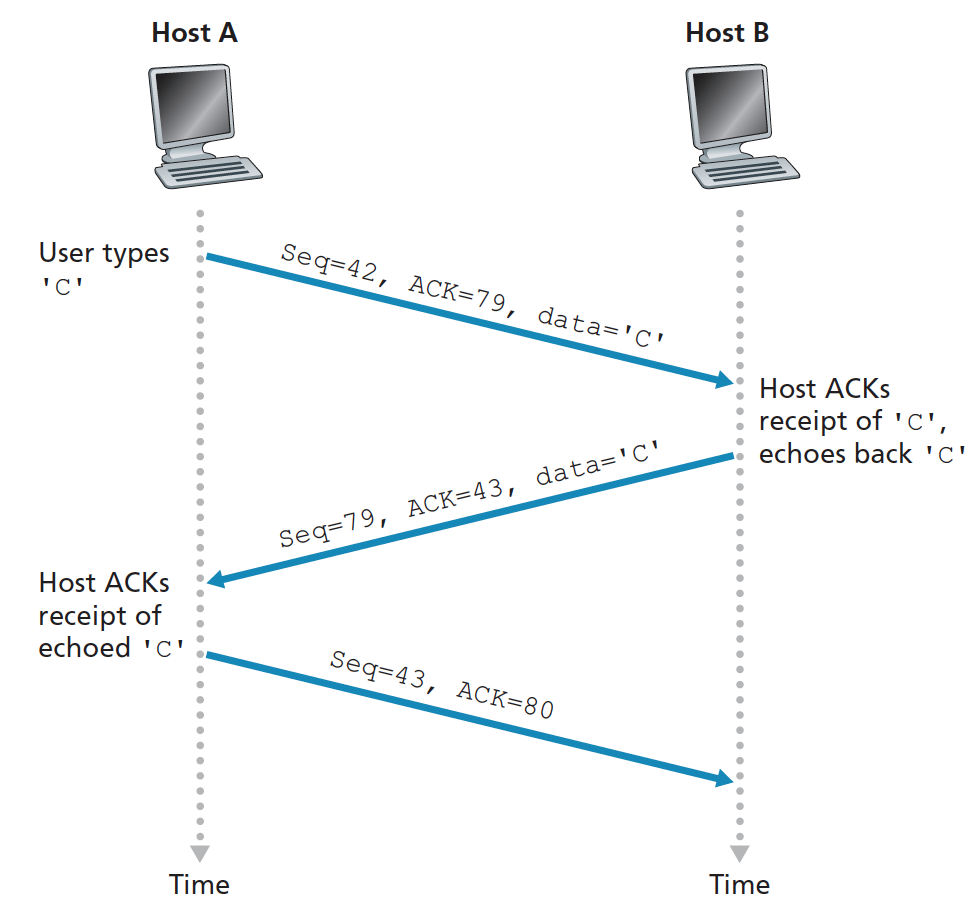
\includegraphics[keepaspectratio, width=15cm, height=12cm]{imagens/12/12 - troca de mensagens tcp.png}
\caption{Sequence number e ACK \\
Imagem retirada de: Computer Networking a top-down approach. 8th
ed.~Pearson, página 234. \\}
\label{Sequence number e ACK}
\end{figure}



\hypertarget{segmentos-fora-de-ordem}{%
\subsubsection{Segmentos fora de ordem}\label{segmentos-fora-de-ordem}}

Como citado anteriormente, o tratamento dos segmentos fora de ordem,
para um sistema confiável de transferência de dados, pode seguir uma
dessas suas estratégias, \emph{GO-BACK-N} ou \emph{Selective Repeat}
(SR). Por uma questão de eficiência, o protocolo SR é a abordagem
praticada.

\hypertarget{rtt-e-timeout}{%
\subsubsection{RTT e Timeout}\label{rtt-e-timeout}}

Depois do envio de um segmento, ao fim de qual intervalo de tempo o TCP
deve considerar que os dados foram perdidos (\texttt{timeout\ interval})
? Esse tempo sofre de uma dicotomia, pois tanto períodos pequenos como
grandes tornam a comunicação ineficiente por causar retransmissões
desnecessárias e aumentar o atraso na retransmissão de segmentos
perdidos, respectivamente.

Podemos considerar que, no mínimo, o tempo esperado deve superar o
\emph{Round-Trip Time} (RTT), período entre o envio de um dado e a
chegada de sua resposta. Como pode-se imaginar, por consequência da não
previsibilidade de uso {[}da rede{]} e da ocorrência de erros, as
condições presentes na rede são variáveis (como um possível
congestionamento), algo que impacta diretamente no (RTT), tornando-o,
também, variável.

Assim, a determinação do \texttt{timeout\ interval} passa por um cálculo
estatístico, definido pelo \texttt{SampleRTT}, uma amostra desse período
medida de tempos em tempos, \texttt{EstimatedRTT}, uma estimativa do
valor do RTT que utiliza a técnica da média móvel exponencialmente
ponderada (EWMA, \emph{Exponential Weighted Moving Average}), e
\texttt{DevRTT}, uma estimativa de quanto o \texttt{SampleRTT} desvia do
\texttt{EstimatedRTT}. Os cálculos podem ser vistos a seguir.

Valores recomendados {[}RFC 6298{]}: α = 0.125 (1/8) β = 0.25 (1/4)

\begin{verbatim}
EstimatedRTT = (1 – α) * EstimatedRTT + α * SampleRTT
\end{verbatim}

\begin{verbatim}
DevRTT = (1 – β) * DevRTT + β * | SampleRTT – EstimatedRTT |
\end{verbatim}

Para questões de eficiência, é interessante manter o valor do
\emph{timeout interval} algo como o valor estimado do RTT
(\texttt{EstimatedRTT}) mais uma margem que se adéque à flutuação de
valor do \texttt{SampleRTT} (\texttt{DevRTT}). Dessa maneira, chegamos
do cálculo a seguir (sendo 1 segundo o valor inicial):

\begin{verbatim}
TimeoutInterval = EstimatedRTT + 4 * DevRTT
\end{verbatim}

\hypertarget{complementar-5}{%
\section{Complementar}\label{complementar-5}}

\hypertarget{pesquisar-sobre-4}{%
\subsection{Pesquisar Sobre}\label{pesquisar-sobre-4}}

\begin{enumerate}
\def\labelenumi{\arabic{enumi}.}
\tightlist
\item
  Flow Control (Computer Networking a top-down approach. 8th
  ed.~Pearson, página 246)
\item
  TCP Connection Management (Computer Networking a top-down approach.
  8th ed.~Pearson, página 249)
\item
  Congestion Control (Computer Networking a top-down approach. 8th
  ed.~Pearson, página 255)
\item
  TCP Congestion Control (Computer Networking a top-down approach. 8th
  ed.~Pearson, página 263) (TCP Cubic, Fairness)
\item
  Evolution of Transport-Layer Functionality (Computer Networking a
  top-down approach. 8th ed.~Pearson, página 279) (QUIC (\emph{Quick UDP
  Internet Connection}))
\end{enumerate}